\documentclass[12]{article}
\usepackage{titlesec}
\usepackage{indentfirst}
\usepackage [english]{babel}
\usepackage [utf8]{inputenc}
\usepackage [T1] {fontenc}
\usepackage{subfiles}
\usepackage{wrapfig}
\usepackage{graphicx}
\usepackage{sidecap}
\usepackage{amssymb}
\usepackage{amsmath}
\usepackage{multirow}
\usepackage[english]{babel}
\graphicspath{ {./images/} }
\usepackage[export]{adjustbox}
\usepackage{enumitem}
\usepackage[absolute,overlay]{textpos}
\usepackage{float}
\usepackage{forest}
\usepackage{amsmath,amsfonts,amsthm,amssymb}
\usepackage{graphicx}
\usepackage{pdfpages}
\usepackage{amsmath}
\addtocontents{toc}{\protect\thispagestyle{empty}}
\usepackage[margin = 2.8 cm, headheight = 1.5pt]{geometry}
\usepackage{hyperref}
\usepackage{graphicx}
\usepackage{siunitx}

\usepackage{colortbl}
\usepackage{textgreek}



\begin{document}


\begin{titlepage}
\includepdf[fitpaper]{title}
\end{titlepage}

\newpage
\tableofcontents
\listoffigures
\newpage
\clearpage
\setcounter{page}{1}


\section*{Introduction}
As part of our APP project, we are taking on the challenge set by Events IT. In this report, our mission is to explore and identify the most efficient telecommunication technologies specifically suited to our festivals. The objective is clear: to guarantee that our sensors communicate through the most efficient channel possible. \\

In this report, we analyze the use of cutting-edge communication technologies to improve the sound atmosphere of outdoor music events. We take into account the hearing health of participants, notably thanks to live feedback provided on site through the user interface. Relying on an in-depth analysis of the technical specifications of the various means of communication such as Bluetooth, Wi-Fi, 4G and optical fiber, the goal is to set up a reliable and efficient system for collecting, processing and distributing data on sound levels, thus ensuring a safe and enriching experience for both users and the organizer. This document aims to establish a constructive dialogue between technology, well-being and innovation. \\

The adoption of these communication technologies in our initiative goes beyond the simple exchange of data. It is an integral part of a larger vision that seeks to enhance the well-being of users while making the organization and management of music events (festivals) more efficient. With particular attention paid to the health of users / spectators, our solution positions itself as a key innovation for developing sound spaces that are both safe and pleasant. This strategy encompasses not only a benefit for participants, by informing them of the risks related to sound exposure, but it is also valuable for organizers. They now have an effective means of monitoring and adjusting the sound volume, guaranteeing a pleasant musical experience. \\


\section{Wireless network specifications}

\subsection{Bluetooth specifications}

The company Events-IT gave us the task of analyzing a file transfer via Bluetooth between two devices. On one side, a smartphone (object) which plays the role of receiver, and on the other a laptop (gateway) which is the transmitter.

We know that the company that assigned us our mission wishes to deploy 35 objects over an area of 400 m². However, a gateway cannot manage an infinite number of objects simultaneously. After some research, we confirmed that the gateway could manage a maximum of 7 objects, so there is 1 master (gateway) for 7 active slaves (objects). To conclude, assuming that all 35 objects are active simultaneously, 5 masters will therefore be needed, each managing 7 slaves.

\subsection{Wi-Fi specifications}

Wi-Fi first appeared in 1987 under the name IEEE 802.11 (the technical name of the Wi-Fi technology).
Since then, like any innovation, it is bound to evolve. In the early years, the usage of the time determined the throughput available to users. However, over time, with the multiplication of connected devices and the democratization of this technology, fiber emerged, theoretically providing a throughput of up to 1.3 Gbit/s (1300 Mbit/s).

Wi-Fi works as a wireless communication protocol, via radio waves defined on the 2.4 GHz or 5 GHz band, which connect devices over short distances. For reliability, bandwidths of 20, 40 or 80 MHz have been put in place. They provide wireless Internet access but also allow the creation of local networks for companies or households.

Here, we will use Wi-Fi to create a local network that will link the previously determined Bluetooth gateways with the central server. After comparison with Bluetooth, the use of Wi-Fi is the most optimized solution thanks to its large geographical coverage. In other words, Wi-Fi can reach much more distant areas in order to cover the entire required zone.

\subsection{Mobile network specifications}
Mobile networks are already considerably developed today; they are advanced systems for data transmission. This transmission is carried out remotely via radio waves over various frequency bands. These networks outperform Wi-Fi and Bluetooth (in particular the 4G and 5G technologies) thanks to their extended coverage and their ability to manage a large number of devices over vast areas. Their infrastructure guarantees increased reliability and security, notably due to reinforced encryption and authentication protocols. \\

The costs associated with mobile networks are often justified by their wide coverage and superior reliability. Despite a higher energy consumption than Bluetooth, the mobile network allows a higher data transfer speed.\\

For our long-term project, we chose to rely on the Bouygues Telecom mobile network, confident in its ability to meet our requirements.



\section{Wired network specifications}

\subsection{Coaxial cable}

A coaxial cable is a link that allows the transmission of digital and analog signals at high or low frequency. It has several functions, notably linking two audio or video devices or connecting an antenna to a TV decoder.

This cable has several characteristics of its own, such as the presence of an outer sheath around the cable to prevent minor physical damage, a copper conductor used to transmit electronic signals and finally a copper braid that serves as a second wire in the circuit and as shielding.

Coaxial cable is optimized for short or medium distances because of the strong attenuation related to the distance traveled by the signals, which is more than 10 dBm/Km.

\subsection{Single-mode optical fiber}

Fiber is the most recent and most powerful means of obtaining a reliable, stable and sufficiently powerful connection. Several types exist; the two main ones are single-mode and multimode, which differ in their characteristics and their uses.

The single-mode type is considered the most powerful; it can be used over very long distances thanks to its small core and its unique method of carrying one mode of light called the transverse mode. In other words, the light entering the fiber propagates along a straight path along the axis of the fiber without being reflected or scattered.
The attenuation of this fiber is almost zero, which is one of its greatest advantages; it is therefore the most popular, notably at the core of worldwide networks, despite its rather high cost.

\subsection{Step-index multimode fiber}

One of the types of multimode fiber is the step-index one; it was the first type of fiber designed. Its core is made entirely of a single type of material. Its operation differs on the principle of total reflection: the incoming light propagates in a zigzag along the axis of the fiber, reflecting each time it meets the cladding of the optical fiber.
However, it has a few drawbacks: a higher attenuation due to the path of the light, and a speed too low for certain uses because of the dispersion related to the path lengths. This type of fiber is not widely used, mainly except for consumer audio and television links.

\subsection{Graded-index multimode fiber}

Finally, the graded-index multimode fiber, which offers hundreds of times more bandwidth than the step-index fiber. It differs from the latter through the composition of the glass in its core, which compensates for the different path lengths of the modes. In other words, the light propagates along curved paths along the axis of the fiber.
Its core being smaller than the previous ones, this allows it to reduce the variations in travel time and the attenuation that could occur over long distances.




\section{General network architecture}

\begin{figure}[H]
    \centering
    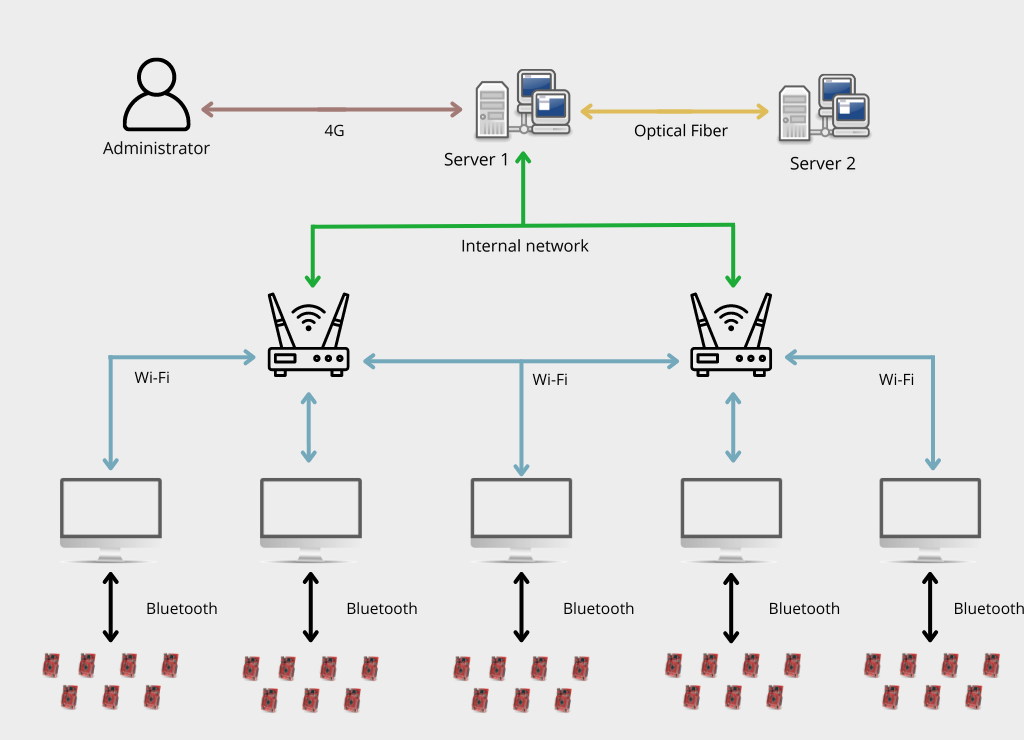
\includegraphics[width=1\linewidth]{1111.png}
    \caption{Overall architecture of the central network}
    \label{fig:enter-label}
\end{figure}

The overall architecture of our central network is laid out as shown above. First, the administrator: they are connected via 4G to a first server and can therefore access all the information on the network. A second server is connected to the first via an optical fiber connection.

The information received by the first server comes from two distinct routers, which transmit their information through the internal network. Connected to these routers are 5 computers that communicate with each other through a Wi-Fi connection.

Finally, 7 sensors are connected via Bluetooth to each of the computers, forming 5 distinct groups for a total of 35 objects. These 7 connected sensors represent the maximum number of devices that can potentially be connected to one single master, as determined earlier. Each group of sensors connected via Bluetooth to a master computer forms a Piconet network.

This complex network architecture makes it possible to manage the different sections efficiently and to ensure secure data transmission between the different devices that make up this network.

\subfile{Livrable_1}

\section{Connection between the administrator and the web server}


\subsection{Specifications of the surrounding mobile infrastructures}

The company Events-IT wishes to offer more flexibility to the administrator in terms of mobility, thus allowing permanent access to the network. In this part, we will explore in more depth the use of wireless technologies to transmit information in an everyday setting. \\

% Question 1
To offer more flexibility in terms of mobility to the administrator, allowing permanent access to the network, 4G LTE technology can be used. This mobile technology allows high-speed connections and is well suited for wireless connections over long distances.\\

% Question 2
4G LTE: The maximum power of the transmitters can vary, but for mobile devices it is generally around 23 dBm. For fixed transmitters (base stations), it can reach up to 46 dBm in some cases. The theoretical maximum throughput of 4G LTE is about 1 Gbps for download and 100 Mbps for upload.

% Question 3
\begin{figure}[H]
    \centering
    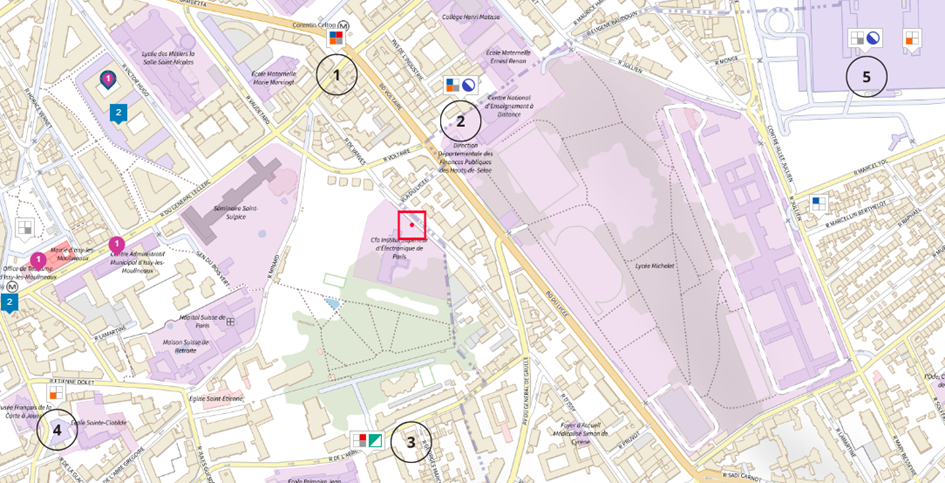
\includegraphics[width=1\linewidth]{image1.png}
    \caption{Map of the antennas close to our location}
    \label{fig:enter-label}
\end{figure}
\begin{itemize}
    \item [$\bullet$] Antenna No. 1: Identification No.: 2055632 \\

Site description: Underground indoor / 0m / RATP \\

Address: PLACE PAUL VAILLANT COUTURIER MÉTRO CORENTIN CELTON L12 \\

Postal code / Municipality: 92130 ISSY LES MOULINEAUX \\

Telephony: Bouygues (3G/4G) ; Orange (3G/4G) ; SFR (2G/3G/4G) ; FREE (3G/4G) \\


    \item [$\bullet$] Antenna No. 2: Identification No.: 1447454 \\

Site description: Building / 38m / Social housing company \\

Address: 35 RUE ERNEST RENAN \\

Postal code / Municipality: 92130 ISSY LES MOULINEAUX \\

Telephony: BOUYGUES (2G/3G/4G/5G) ; ORANGE (2G/3G/4G/5G) ; FREE (3G/4G/5G) \\

    \item [$\bullet$] Antenna No. 3: Identification No.: 1903324 \\

Site description: Building / 23m / Social housing company \\

Address: 11 R DE L'ABBÉ DERRY \\

Postal code / Municipality: 92130 ISSY LES MOULINEAUX \\

Telephony: SFR (2G/3G/4G/5G) ; FREE (3G/4G/5G) \\

    \item [$\bullet$] Antenna No. 4: Identification No.: 460465 \\

Site description: Building / 37m / Social housing company \\

Address: 13 B R AUGUSTE GERVAIS \\

Postal code / Municipality: 92130 ISSY LES MOULINEAUX \\

Telephony: ORANGE (2G/3G/4G/5G) \\

    \item [$\bullet$] Antenna No. 5: Identification No.: 2027208 \\

Site description: Building / 36m / Municipality, community of municipalities \\

Address: 2 RUE DU 4 SEPTEMBRE \\

Postal code / Municipality: 92170 VANVES \\

Telephony: FREE (3G/4G/5G) \\


\end{itemize}

\subsection{Focus on one antenna}

% Question 4

The antennas to which the administrator's smartphone is connected are equipped with 2G, 3G, 4G and 5G technologies, microwave links and BLR LTE 3500 (a very high speed wireless transmission technology used while waiting for fiber to be deployed everywhere).
Most of the antennas are installed on buildings, some in the metro at the Corentin Celton station. The majority of the antennas carry infrastructures belonging to several Internet service providers.

The one to which my phone is most likely connected has the identification number 1903324. It is located on the roof of a social housing building at 11 rue de l'abbé Derry, in Issy-les-Moulineaux. It provides 2G, 3G, 4G and 5G services for SFR, 3G, 4G and 5G services for Free, and a BLR LTE 3500 antenna (very high speed wireless).

% Question 5

We now want to calculate the radius of the safety zone for the 1800 MHz mobile telephony band.

We consider the antenna gain formula:
\begin{equation*}
    \text{G}_\text{A}(\theta)[dB] = \text{G}_\text{max}[dB] - min\left(12\left(\frac{\theta}{\theta_{3dB}}\right)^2,20\right)
\end{equation*}

With
\begin{itemize}
    \item [$\bullet$] $\text{G}_{max}[dB] = 17dB$ the maximum gain of the antenna
    \item [$\bullet$] $\theta_{3dB} = \text{\ang{70}}$ \\
\end{itemize}

To calculate the gain of our antenna, we must determine the angle of our position with respect to its transmission angle. To do this, we carry out angle measurements with the cartoradio tool (cf. sources), as follows: \\

We use the east-west axis as a reference. With respect to it, we measure the angle of the antennas of interest. We find an angle of \ang{40} (figure~\ref{fig:antouest}) with respect to our reference axis for the one transmitting towards the west, and \ang{21} (figure~\ref{fig:antest}) for the one transmitting towards the east.

\begin{figure}[H]
    \centering
    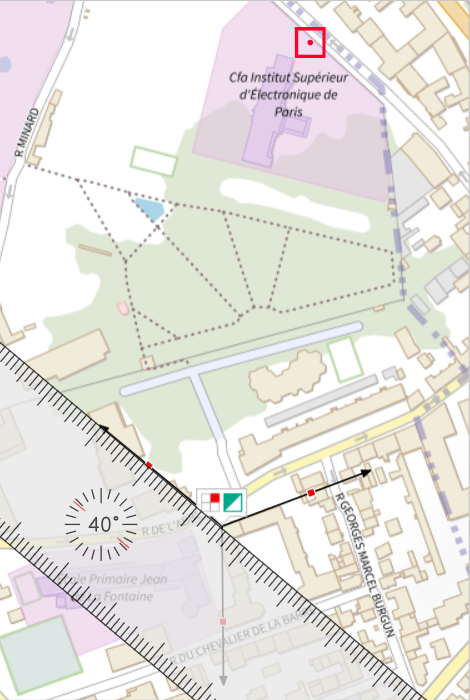
\includegraphics[width=0.3\linewidth]{antenneouest.png}
    \caption{Angle of the antenna transmitting towards the west}
    \label{fig:antouest}
\end{figure}

\begin{figure}[H]
    \centering
    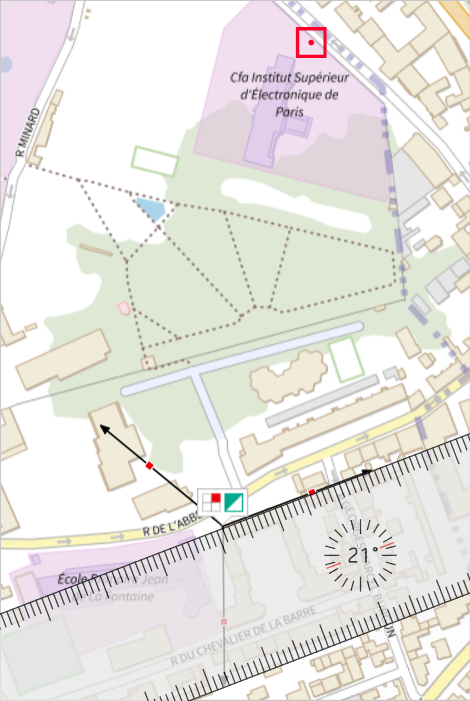
\includegraphics[width=0.3\linewidth]{antenneest.png}
    \caption{Angle of the antenna transmitting towards the east}
    \label{fig:antest}
\end{figure}

To determine which antenna provides the best quality of service given my position, we determine the angle between these two antennas, then the bisector of this angle:

\begin{equation*}
    180 - (40 + 21) = 119
\end{equation*}

\begin{equation*}
    \frac{119}{2} = \ang{59.5} \approx \ang{60}
\end{equation*}

If we plot this angle on the map ($80 = 180 - (60 + 40)$), we can see that the antenna providing the best quality of service is the one transmitting towards the west (figure~\ref{fig:antbissec}).

\begin{figure}[H]
    \centering
    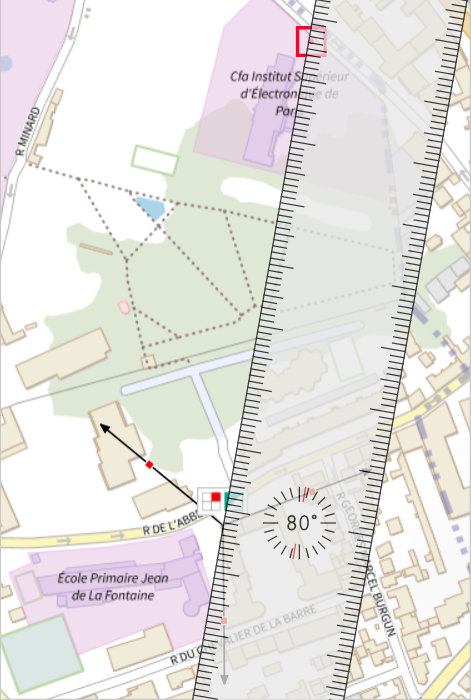
\includegraphics[width=0.3\linewidth]{bissecantennes.png}
    \caption{Bisector of the antenna angles}
    \label{fig:antbissec}
\end{figure}

By slightly shifting the angle measurement, we find that my position is at \ang{81} with respect to the reference axis. We therefore find an angle of \ang{39} between the antenna and my position.

With these parameters, we determine the gain of the antenna by the numerical application of the formula given above, knowing that $\theta = \ang{39}$:

\begin{equation*}
    \text{G}_\text{A}(39)[dB] = 17 - min\left(12\left(\frac{39}{70}\right)^2,20\right)
\end{equation*}

\begin{equation*}
    12 \times \left(\frac{39}{70}\right)^2 = 3.724897959 \approx 3.72
\end{equation*}

\begin{equation*}
    \text{G}_\text{A}(39)[dB] = 17 - min(3.72,20)
\end{equation*}

\begin{equation*}
    \text{G}_\text{A}(39)[dB] = 17 - 3.72 = 13.28dB
\end{equation*}

The antenna has a gain of 13.28dB. We now look for the value of the electric field of the antenna. We take the electric field strength values for the 4G frequency bands covered by our antenna.

\begin{table}[H]
\centering
\resizebox{0.6\columnwidth}{!}{%
\begin{tabular}{|c|c|}
\hline
\rowcolor[HTML]{000000}
{\color[HTML]{FFFFFF} Frequency band (MHz)} & {\color[HTML]{FFFFFF} Electric field strength (V/m)} \\ \hline
700 & 38 \\ \hline
800 & 39 \\ \hline
1800 & 59 \\ \hline
2100 & 61 \\ \hline
2600 & 61 \\ \hline
\end{tabular}%
}
\end{table}

We use this relation to measure the electric field of our antenna:

\begin{equation*}
    \sum_{f_{i}} \left(\frac{E_{i}}{E_{l}(f_{i})}\right)^2 \leq 1
\end{equation*}

By isolating the electric field and adding the numerical values, we find this inequality:

\begin{equation*}
    E_{i}^2\left(\frac{1}{38^2} + \frac{1}{39^2} + \frac{1}{59^2} + \frac{1}{61^2} + \frac{1}{61^2} \right) \leq 1
\end{equation*}

We know that:

\begin{equation*}
    \text{E} = \sqrt{\frac{P_{e} G_{e} Z_{0}}{4 \pi d^2}}
\end{equation*}

We therefore have:

\begin{equation*}
    E_{i}^2 = \frac{P_{e} G_{e} Z_{0}}{4 \pi d^2}
\end{equation*}

We take $P_{e} \times G_{e} = 13161 W$, which we divide by 5 to find the average transmission power over the 4G antennas ($\frac{13161}{5} = 2632.2 W)$ and we substitute it into the formula found above:

\begin{equation*}
   \frac{2632.2 \times 377}{4 \pi} \left(\frac{1}{38^2} + \frac{1}{39^2} + \frac{1}{59^2} + \frac{1}{61^2} + \frac{1}{61^2}\right) \leq d^2
\end{equation*}

We can now carry out the numerical application to find the safety distance:

\begin{equation*}
    d = \sqrt{\frac{2632.2 \times 377}{4 \pi} \left(\frac{2}{61^2} + \frac{1}{38^2} + \frac{1}{39^2} + \frac{1}{59^2} \right)}
\end{equation*}

The radius of the safety zone is $d \approx 13.10m$. \\

% Question 6

We are now interested in the EIRP of the base station to which my mobile phone is connected. We use as a reference a screenshot of the NetMonster application (figure~\ref{fig:netmonsterpire}).

\begin{figure}[H]
    \centering
    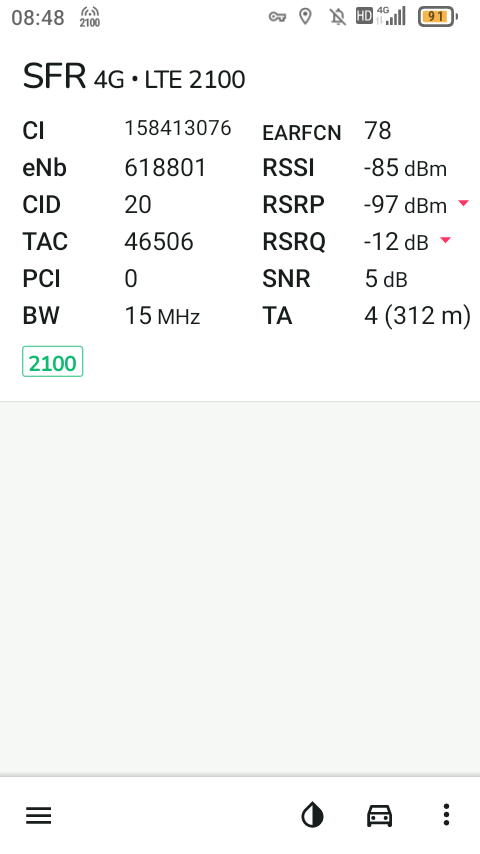
\includegraphics[width=0.3\linewidth]{screenshot_netmonster.png}
    \caption{Screenshot of the NetMonster application}
    \label{fig:netmonsterpire}
\end{figure}

First of all, we will take as the received power level an average of the RSSI over four measurements. The carrier frequency of the signal is 2100 MHz. The measurements taken are available in the following table:


\begin{table}[H]
\centering
\begin{tabular}{|l|l|l|l|l|}
\hline
\rowcolor[HTML]{000000}
{\color[HTML]{FFFFFF} Measurement} & {\color[HTML]{FFFFFF} 1} & {\color[HTML]{FFFFFF} 2} & {\color[HTML]{FFFFFF} 3} & {\color[HTML]{FFFFFF} 4} \\ \hline
RSSI (dBm) & -89 & -93 & -91 & -87 \\ \hline
RSSI (W) & $1.26\times10^-12$ & $5.01\times10^-13$ & $7.94\times10^-13$ & $1.99\times10^-12$ \\
\hline
\end{tabular}
\end{table}

We find an average of 90dBm for the RSSI. To find the value of the EIRP, we use this relation: EIRP [dBm] - RSSI[dBm] = Attenuation [dBm] \\

To find the transmission power, we use the attenuation formula of the Okumura-Hata model:

\begin{equation*}
    A_{p} = 46.3 + 33.9 \times log_{10}(f) - 13.82 \times log_{10}(h_{b}) + (44.9 - 6.55 \times log_{10}(h_{b}) )\times log_{10}(d) - a(h_{m}) + C_{m} \\
\end{equation*}

With $a(h_{m})$:

\begin{equation*}
    a(h_{m}) = 3.2 log_{10}(11.75 h_{m})^2 - 4.97
\end{equation*}

We take the following parameters:

\begin{itemize}
    \item $f = 2600$ : The carrier frequency
    \item $h_{b} = 23m$ : The height of the antenna
    \item $h_{m} = 9m$ : The height of the mobile phone
    \item $C_{m} = 3dB$
    \item $d = 280m$ : Distance measured via cartoradio between the antenna and the mobile
\end{itemize}

We carry out the numerical application to find $a(h_{m})$:

\begin{equation*}
    a(h_{m}) = 3.2 log_{10}(11.75 \times 9)^2 - 4.97
\end{equation*}

\begin{equation*}
    a(h_{m}) = 8.14
\end{equation*}

We now carry out the numerical application to find $A_{p}$:

\begin{equation*}
    A_{p} = 46.3 + 33.9 \times log_{10}(2600) - 13.82 \times log_{10}(23) + (44.9 - 6.55 \times log_{10}(23) )\times log_{10}(280) - 8.14 + 3
\end{equation*}

\begin{equation*}
    A_{p} = 226.16 dBm
\end{equation*}

We now use the relation stated earlier, which is: EIRP [dBm] - RSSI[dBm] = Attenuation [dBm]

EIRP [dBm] = RSSI [dBm] + Attenuation [dBm]

By carrying out the numerical application, we find:

\begin{equation*}
    \text{EIRP [dBm]} = -90 + 226.16 = 136.016
\end{equation*}

We deduce the transmission power:

\begin{equation*}
    P_{e} = EIRP - G_{A}(39)[dB] = 136.016 - 13.28 = 122.736 dBm
\end{equation*}

The calculated power corresponds to one resource block (RB). To find the EIRP of the base station, it must be multiplied by the number of RBs corresponding to the observed bandwidth. We find a bandwidth of 15 MHz, so we have 75 RBs. By calculating, we find:

\begin{equation*}
    P_{e}(75) = 122.736 + 10 log_{10}(75) = 141.49 dBm
\end{equation*}

The transmission power is 141.49 dBm.

\section{Optical fiber and cables}

As part of the mission given to us by Events-IT, we are looking to connect several centers by wire in the most optimized way. We wish to ensure the best throughput, knowing that the centers are located about 50 kilometers from each other. Several solutions exist to provide a high-speed wired connection. In our case, we will focus on four distinct technologies: coaxial cable, step-index multimode fiber, graded-index multimode fiber and single-mode fiber.

First of all, we compared some characteristics of these tools in the table below:


\begin{table}[H]
\centering
\begin{tabular}{
>{\columncolor[HTML]{000000}}c |l|l|l|l|}
\cline{2-5}
 & \multicolumn{1}{c|}{\cellcolor[HTML]{000000}{\color[HTML]{FFFFFF} \textbf{Bandwidth}}} & \multicolumn{1}{c|}{\cellcolor[HTML]{000000}{\color[HTML]{FFFFFF} \textbf{\begin{tabular}[c]{@{}c@{}}Transmitted \\ power\end{tabular}}}} & \multicolumn{1}{c|}{\cellcolor[HTML]{000000}{\color[HTML]{FFFFFF} \textbf{Attenuation}}} & \multicolumn{1}{c|}{\cellcolor[HTML]{000000}{\color[HTML]{FFFFFF} \textbf{Range and throughput}}} \\ \hline
\multicolumn{1}{|c|}{\cellcolor[HTML]{000000}{\color[HTML]{FFFFFF} Coaxial}} & 12 to 60 MHz& 2.3 W & 10 dB/km& \begin{tabular}[c]{@{}l@{}}Short distance (consumer \\ use and max 1Gb/s)\end{tabular} \\ \hline
\multicolumn{1}{|c|}{\cellcolor[HTML]{000000}{\color[HTML]{FFFFFF} Single-mode}} & 1 THz (infinite)& 1 to 10 W& 0.5 dB/km& \begin{tabular}[c]{@{}l@{}}Long distance and high throughput\\ +100km\end{tabular} \\ \hline
\multicolumn{1}{|c|}{\cellcolor[HTML]{000000}{\color[HTML]{FFFFFF} \begin{tabular}[c]{@{}c@{}}Step-index\\ multimode\end{tabular}}} & 20 to 100 MHz& 1 to 10 W& 4-6 dB/km& \begin{tabular}[c]{@{}l@{}}Short distance (a few km\\ and reduced speed 8 mb/s)\end{tabular} \\ \hline
\multicolumn{1}{|c|}{\cellcolor[HTML]{000000}{\color[HTML]{FFFFFF} \begin{tabular}[c]{@{}c@{}}Graded-index\\ multimode\end{tabular}}} & 2 GHz& 1 to 10 W& 3 dB/km& \begin{tabular}[c]{@{}l@{}}Medium distance (10 - 20 km \\ and high speed 40 - 140 Mb/s)\end{tabular} \\ \hline
\end{tabular}
\end{table}

\subsection{Characteristics of the different mediums}

We now look for which solution would be the most suitable for our transmission distance. To do this, we first look for the received power and then deduce the maximum transmission distance for each of the mediums.


\subsubsection{Coaxial cable}

\begin{equation*}
    C = B \times \log_2 \left( \text{SNR} + 1 \right)
\end{equation*}

\begin{equation*}
    \text{SNR} = 2^{\frac{C}{B}} - 1
\end{equation*}

\begin{equation*}
    \text{SNR} = 2^{ \frac{10^9}{6 \times 10^7}} -1 = 104030.9
\end{equation*}

\begin{equation*}
    \text{SNR} = \frac{RSSI}{P_e}
\end{equation*}

\begin{equation*}
    P_r = SNR \times KTB
\end{equation*}

\begin{equation*}
    P_r = 104031 \times 1.38.10^{-23} \times 290 \times 6.10^7
\end{equation*}

\begin{equation*}
    P_r = 2.5.10^{-8} \text{ W} = -76 \text{ dBm}
\end{equation*}

We deduce the maximum transmission distance:

\begin{equation*}
    d = \frac{Att}{Att_{dB/km}}
\end{equation*}

\begin{equation*}
    P_e = 2.3 \text{ W} = -26.3827 \text{ dBm}
\end{equation*}

\begin{equation*}
    Att = P_e - P_r
\end{equation*}

\begin{equation*}
    Att = -26.3827 - \left( -76 \right) = 49.6173 \text{ dBm}
\end{equation*}

\begin{equation*}
    d = \frac{49.6173}{10} = 4.96173 \text{ km} \approx 4.96 \text{ km}
\end{equation*}

The maximum transmission distance of the coaxial cable is therefore 4.96 km.


\subsubsection{Single-mode fiber}

For fiber we have RSSI $= P_r$ because the reflection coefficient is zero.


\begin{equation*}
    \text{SNR} = 2^{ \frac{10^9}{10^{12}}} -1 = 0.000693
\end{equation*}

\begin{equation*}
    P_r = 0.000693 \times 1.38.10^{-23} \times 290 \times 10^{12}
\end{equation*}

\begin{equation*}
    P_r = 2.77.10^{-12} \text{ W} = -120 \text{ dBm}
\end{equation*}

We deduce the maximum transmission power:

\begin{equation*}
    d = \frac{Att}{Att_{dB/km}}
\end{equation*}

\begin{equation*}
    P_e = 10 \text{ W} = 40 \text{ dBm}
\end{equation*}

\begin{equation*}
    Att = P_e - P_r
\end{equation*}

\begin{equation*}
    Att = 40 - \left( -120 \right) = 160 \text{ dBm}
\end{equation*}

\begin{equation*}
    Range = \frac{160}{0.5} \approx 320 \text{ km}
\end{equation*}

The maximum transmission distance of a single-mode optical fiber cable is therefore 320 km.

\subsubsection{Step-index multimode fiber}


\begin{equation*}
    \text{SNR} = 2^{ \frac{10^9}{10^{8}}} -1 = 1023
\end{equation*}

\begin{equation*}
    P_r = 1023 \times 1.38.10^{-23} \times 290 \times 10^{8}
\end{equation*}

\begin{equation*}
    P_r = 4.09^{-10} \text{ W} = -63.88 \text{ dBm}
\end{equation*}

We deduce the maximum transmission distance:

\begin{equation*}
    d = \frac{Att}{Att_{dB/km}}
\end{equation*}

\begin{equation*}
    P_e = 10 \text{ W} = 40 \text{ dBm}
\end{equation*}

\begin{equation*}
    Att = P_e - P_r
\end{equation*}

\begin{equation*}
    Att = 40 - \left( -63.88 \right) = 103.88 \text{ dBm}
\end{equation*}

\begin{equation*}
    d = \frac{103.88}{6} \approx 17.31 \text{ km}
\end{equation*}

The maximum transmission distance of a step-index multimode optical fiber cable is therefore 17.31 km.


\subsubsection{Graded-index multimode fiber}


\begin{equation*}
    \text{SNR} = 2^{ \frac{10^9}{2 \times 10^{9}}} -1 = 0.414214
\end{equation*}

\begin{equation*}
    P_r = 1 \times 1.38.10^{-23} \times 290 \times 2 \times 10^{9}
\end{equation*}

\begin{equation*}
    P_r = 3.315^{-12} \text{ W} = -84.79 \text{ dBm}
\end{equation*}

We deduce the maximum transmission distance:

\begin{equation*}
    d = \frac{Att}{Att_{dB/km}}
\end{equation*}

\begin{equation*}
    P_e = 10 \text{ W} = 40 \text{ dBm}
\end{equation*}

\begin{equation*}
    Att = P_e - P_r
\end{equation*}

\begin{equation*}
    Att = 40 - \left( -84.79 \right) = 124.79 \text{ dBm}
\end{equation*}

\begin{equation*}
    d = \frac{124.79}{3} \approx 41.598 \text{ km}
\end{equation*}

The maximum transmission distance of a graded-index multimode optical fiber cable is therefore 41.598 km.

\newpage
\subsection{Comparison and recommended solution}

\begin{figure}[H]
    \centering
    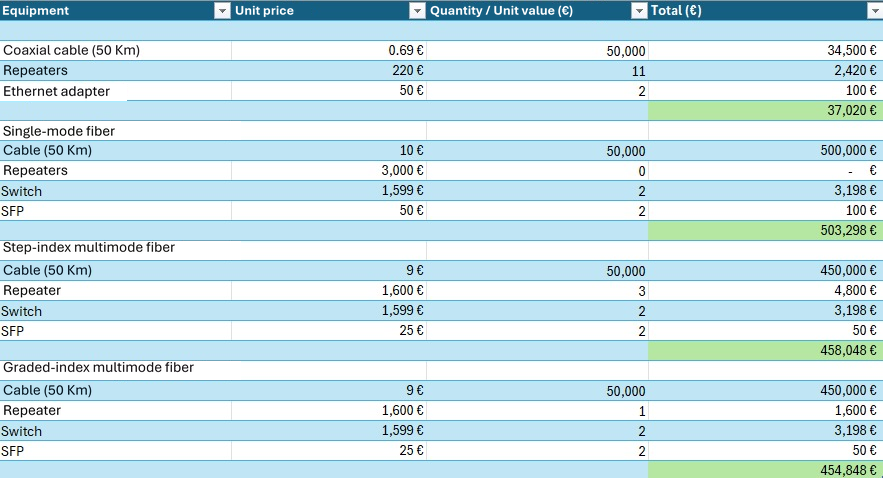
\includegraphics[width=1\linewidth]{image.png}
    \caption{Price table of the different mediums and equipment}
    \label{fig:enter-label}
\end{figure}

\begin{table}[H]
\resizebox{\textwidth}{!}{%
\begin{tabular}{|
>{\columncolor[HTML]{000000}}c |c|c|c|c|}
\hline
\multicolumn{1}{|l|}{\cellcolor[HTML]{000000}{\color[HTML]{FFFFFF} Wired technology}} & \multicolumn{1}{l|}{\cellcolor[HTML]{000000}{\color[HTML]{FFFFFF} Coaxial cable}} & \multicolumn{1}{l|}{\cellcolor[HTML]{000000}{\color[HTML]{FFFFFF} Single-mode optical fiber}} & \cellcolor[HTML]{000000}{\color[HTML]{FFFFFF} \begin{tabular}[c]{@{}c@{}}Graded-index Multimode \\ optical fiber\end{tabular}} & \cellcolor[HTML]{000000}{\color[HTML]{FFFFFF} \begin{tabular}[c]{@{}c@{}}Step-index Multimode\\ optical fiber\end{tabular}} \\ \hline
{\color[HTML]{FFFFFF} Bandwidth} & 12 to 60 MHz & 1 THz & 20 to 100 MHz & 2 GHz \\ \hline
{\color[HTML]{FFFFFF} Received power} & -76 dBm & -120 dBm & -63.88 dBm & -84.79 dBm \\ \hline
{\color[HTML]{FFFFFF} Distance} & 4.96 Km & 320 Km & 17.31 Km & 41.598 Km \\ \hline
{\color[HTML]{FFFFFF} Attenuation} & 10 dB/Km & 0.5 dB/Km & 4-6 dB/Km & 3 dB/Km \\ \hline
{\color[HTML]{FFFFFF} Repeaters} & 11 & 0 & 3 & 1 \\ \hline
{\color[HTML]{FFFFFF} Price} & 37 020 € & 503 298 € & 454 848 € & 458 048 € \\ \hline
\end{tabular}%
}
\end{table}


After a detailed economic and practical analysis, shown above, we advise our client to choose the graded-index multimode fiber. This recommendation is the result of a reflection on the cost-performance ratio. Although its price is slightly higher, the graded-index multimode fiber stands out from the step-index multimode fiber through a better bandwidth, which translates into higher data transmission rates. In addition, it guarantees a more reliable signal transmission over longer distances. Taking these advantages into account, opting for the graded-index multimode fiber constitutes a strategic investment.

\newpage
\section*{Conclusion}

In conclusion, our analysis as well as our experimental measurements have allowed us to better understand the different wireless communication technologies. We compared technologies such as Wi-Fi and Bluetooth and determined the advantages and disadvantages of each of these communication methods. The use of one or the other of these methods therefore requires a careful evaluation according to specific needs.\\

First, Bluetooth: it ensures reliable communication over a reduced perimeter, so it excels at interconnecting personal devices. It also stands out for its ease of setup, and its ability to interconnect devices even those without screens or keyboards. However, as we were able to see during our experiments, it has limits in terms of data transfer speed, so its use must be carefully considered and limited to specific cases.\\

Then, Wi-Fi offers a higher transmission speed, even over a large distance. It is therefore more versatile than Bluetooth and remains usable even for projects that are very demanding in terms of bandwidth. However, it is essential to choose a coherent channel in order to limit noise and interference and thus ensure a stable connection. Its setup is also more complex and more expensive than a Bluetooth connection network.\\

Here, we focus mainly on wireless connection methods, but it is possible to make a connection more stable and improve its throughput by using a wired connection. The speed and stability of this connection can be further improved by using more recent technologies such as optical fiber, for example. \\

In summary, there is no technology that is better than another; each has its weaknesses and strengths. It is necessary to think about the network infrastructure that one wants to set up and decide on a case-by-case basis which solution to use.\\

In our case, and to ensure the proper functioning of our digital solution at the various festival locations, we chose to mix these technologies. Thus, the administrators and the technical team will use a Wi-Fi connection to connect to the web server, and the various sensors present at the festival site will be connected via Bluetooth. The festival-goers, for their part, will be connected to the Internet and will give us their feedback through 4G or 5G. Note that, depending on the layout and size of the different festivals, the architecture of our network could be subject to change.



\newpage
\section*{Sources}

\begin{itemize}{\textwidth}
    \item [$\bullet$] \href{http://f5ad.free.fr/ANT-QSP_F5AD_Pertes-ROS-cable-coaxial.htm}{Coaxial cable - Specifications}

    \item [$\bullet$] \href{https://community.fs.com/fr/article/understanding-fiber-loss-what-is-it-and-how-to-calculate-it.html}{Understanding Fiber Loss and how to calculate it}

    \item [$\bullet$] \href{https://www.optcore.net/fr/single-mode-vs-multimode-fiber-difference/}{Single-mode vs multimode fiber, what is the difference?}

    \item [$\bullet$]\href{https://www.thefoa.org/FR/Chapitre%205.htm#:~:text=La%20fibre%20multimode%20%C3%A0%20gradient,jusqu'%C3%A0%20environ%202%20gigahertz}{Graded-index fiber}

    \item [$\bullet$] \href{https://www.cartoradio.fr}{Map of radioelectric sites and measurements in France}

    \item [$\bullet$] \href{https://www.bag.admin.ch/dam/bag/fr/dokumente/str/nis/faktenblaetter-emf/faktenblatt-bluetooth.pdf.download.pdf/faktenblatt%20bluetooth%20f.pdf}{Bluetooth Class PDF}

\end{itemize}








\end{document}
